\subsection{Pattern recognition}
\label{Sect:SciFiPatRec}

\subsubsection{Straight-line pattern recognition}
\label{SubSect:SciFiSLPatRec}

In the absence of a magnetic field, the tracks passing through the tracker may be described using a straight line in three dimensions. Taking the $z$ coordinate as the independent parameter, the track parameters may be taken to be:

\begin{equation}
 {\bf v^{\rm sl}} =
 \left( 
   \begin{array}{c}
     x_0 \\
     y_0 \\
     t_x \\
     t_y
   \end{array}
 \right)\,;
\end{equation}
where, $x_0$ and $y_0$ are the position at which the track crosses the tracker reference surface, $t_x = \frac{dx}{dz}$ and $t_y = \frac{dy}{dz}$. The track model may then be written:

\begin{eqnarray}
  x & = & x_0 + z t_x {\rm;~and} \\
  y & = & y_0 + z t_y \,.
\end{eqnarray}
Pattern recognition then proceeds as follows. A space-point is chosen in each of two stations, $i$ and $j$ where $i$ and $j$ label two different stations and $j>i$. Ideally, $i=1$ and $j=5$. However, a search of all combinations of pairs for which $j-i>1$ is made, taking the pairs in the order of decreasing separation in $z$; i.e. in order of decreasing $\Delta z_{ji} = z_j - z_i$. Initial values for the track parameters,

\begin{equation}
 {\bf v^{\rm sl}_{\rm Init}} =
 \left( 
   \begin{array}{c}
     x_0^{\rm Init} \\
     y_0^{\rm Init} \\
     t_x^{\rm Init} \\
     t_y^{\rm Init}
   \end{array}
 \right)\,,
\end{equation}
are then calculated as follows:

\begin{eqnarray}
  t_x^{\rm Init} & = & \frac{x_j - x_i}{z_j - z_i} \,;        \\
  x_0^{\rm Init} & = & x_i - z_i t_x^{\rm Init}      \,;        \\
  t_y^{\rm Init} & = & \frac{y_j - y_i}{z_j - z_i} \,; {\rm~and} \\
  y_0^{\rm Init} & = & y_i - z_i t_y^{\rm Init} \,;
\end{eqnarray}
where $(x_i, y_i, z_i)$ are the coordinates of space-point $i$, etc. A search is then made for space-points in each of the stations, $k$, between station $i$ and station $j$. The distance between the $x$ and $y$ coordinates of the space-points in the stations $k;\,j<k<i$ and the line defined by the initial track parameters is then calculated at the reference surface of station $k$ as follows:

\begin{eqnarray}
  \delta x_k & = & x_k - (x_0^{\rm Init} + z_k t_x^{\rm Init}) {\rm~and} \\
  \delta y_k & = & y_k - (y_0^{\rm Init} + z_k t_y^{\rm Init}) \,.
\end{eqnarray}
Points are accepted as part of a ``trial'' track if:

\begin{eqnarray}
  | \delta x_k | & < & \Delta_x {\rm~and} \\
  | \delta y_k | & < & \Delta_y \,.
\end{eqnarray}
If at least one space-point satisfies this selection, a ``trial track'' is formed consisting of the space-points selected in stations $i$, $k$, ... and $j$. For each ``trial track'', a straight-line fit is performed to calculate the fit $\chi^2$:

\begin{equation}
  \chi^2 = \chi_x^2 + \chi_y^2 \,.
\end{equation}
If the fit $\chi^2$ satisfies:
% Expressions for the evaluation of $\chi^2_x$ and $\chi^2_y$ are given in Appendix~\ref{App:LS-SL-fit}. 

\begin{equation}
  \frac{\chi^2}{N-2} < \chi^2_{\rm cut} \,,
\end{equation}
then the trial track is accepted. % and the pattern-recognition track parameters and covariance matrix are calculated using the expressions given in Appendix \ref{App:LS-SL-fit}.

\subsubsection{Helix pattern recognition}
\label{SubSect:SciFiHelicalPatRec}

\paragraph{Helix parameters}

In the presence of a magnetic field, the tracks passing through the tracker may be described using a helix. In tracker coordinates, the tracks form circles in the $(x, y)$ plane. Defining $s$ to be the length of the arc swept out by the track in the $(x, y)$ plane, a track may be described using a straight line in the $(s, z)$ plane. Taking the $z$ coordinate as the independent parameter, the track parameters may be taken to be:

\begin{equation}
 {\bf v^{\rm hlx}} =
 \left( 
   \begin{array}{c}
     x_0    \\
     y_0    \\
     \psi_0 \\
     t_s    \\
     \rho
   \end{array}
   \right)\,;
\end{equation}
where, $x_0$ and $y_0$ are the position at which the track crosses the tracker reference surface, $\psi_0$ is the azimuthal angle of the line tangent to the track in the $(x, y)$ plane, $t_s = \frac{ds}{dz}$ and $\rho$ is the radius of curvature. The angle $\psi_0$ is chosen such that:

\begin{equation}
  {\bf \hat{\psi}_0} = {\bf \hat{k}} \times {\bf \hat{r}} \, ;
\end{equation}
where ${\bf \hat{r}}$ is the unit vector in the direction $(x_0, y_0)$ and ${\bf \hat{k}}$ is the unit vector parallel to the $z$ axis. ${\bf \hat{\psi}_0}$ is the unit vector tangent to the track and in the direction is defined by $\psi_0$. With this definition, the projection on the $(x, y)$ plane of a positive track propagating in the positive $z$ direction sweeps anticlockwise.

\paragraph{Track model for pattern recognition}

To build up the track model, consider a track-based coordinate system which has its origin at the point $(x_0, y_0)$ and in which the $x'$ axis is parallel to the line joining $(x_0, y_0)$ to the centre of the circle described by the track, the $y'$ axis is parallel to ${\bf \hat{\psi}_0}$ and the $z'$ axis is parallel to ${\bf \hat{k}}$ (see figure \ref{Fig:PatRecTrkMdl}).

A point, $i$, on the track at $(x_i, y_i)$ (tracker coordinates) at which the track direction is $\psi_i$ may be used to write down the track model as:

\begin{eqnarray}
  x'_i & = & \rho [ \cos\phi'_i - 1 ] {\rm~and} \\
  y'_i & = & \rho \sin\phi'_i \,;
\end{eqnarray}
where:

\begin{equation}
  \tan \frac{\phi'_i}{2} = 
                       \frac{\sqrt{(x_i - x_0)^2 + (y_i - y_0)^2}}
                       {2\rho} \, .
\end{equation}
The $z$ coordinate is taken as a parameter since the construction of the trackers ensures that each reference surface (tracker, station or doublet layer) is at a well defined $z$. The distance travelled in the $(x, y)$ plane to reach the $i^{\rm th}$ point, $s_i$, is related to the $z$ coordinate of the $i^{\rm th}$ point by:

\begin{equation}
  s_i = t_s z_i \, ;
  \label{Eq:sFnz}
\end{equation}
since the track is refered to the tracker reference surface. The transformation from the primed to tracker coordinates is achieved with a rotation, $\underline{\underline{R}}'$, through an angle $-\beta$ and a translation, $\underline{\underline{T}}'$ from $(x_0, y_0)$ to $(0, 0)$:

\begin{equation}
  \left(
      \begin{array}{cc}
         x                                                         \\
         y
      \end{array}
  \right)                 =
  \underline{\underline{T}}' + \underline{\underline{R}}'
  \left(
      \begin{array}{cc}
         x'                                                        \\
         y'
      \end{array}
  \right) \, .
\end{equation}
These transformations are given by:

\begin{eqnarray}
  \underline{\underline{R}}' & = & 
    \left( 
      \begin{array}{cc}
         \cos \beta & -\sin \beta \\
         \sin \beta & \cos \beta 
      \end{array}
    \right) \, ; {\rm and}                                         \\
  \underline{\underline{T}}' & = &
    \left( 
      \begin{array}{c}
         -x_0  \\
         -y_0 
      \end{array}
    \right) \, ;                                                  \\
\end{eqnarray}
where:

\begin{equation}
  \beta = \psi_0 - \frac{\pi}{2} \, .
\end{equation}
\begin{figure}
  \begin{center}
    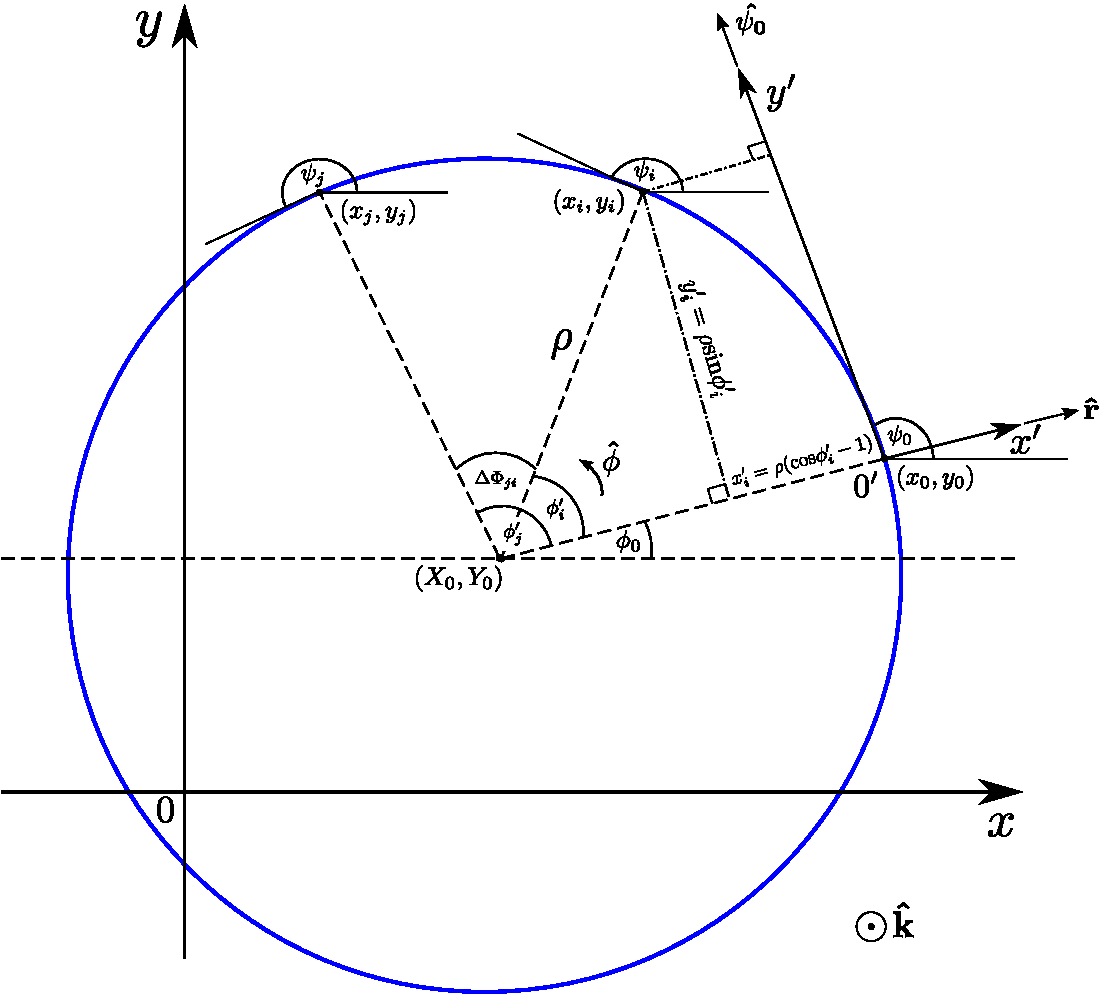
\includegraphics[width=0.85\linewidth]{detectors/tracker/04-Reconstruction/04-03-Pattern-recognition/Figures/Track-model.pdf}
  \end{center}
  \caption{Schematic diagram of track in $(x, y)$ plane.}
  \label{Fig:PatRecTrkMdl}
\end{figure}

\paragraph{Collecting space-points in the $(x, y)$ plane}

Helix pattern recognition follows the same conceptual steps as the straight-line pattern recognition described in section \ref{SubSect:SciFiSLPatRec} A space-point is chosen in each of three stations, $i$, $j$ and $k$ where $k>j>i$. Ideally, $i=1$, $j=3$ and $k=5$. However, a search of all combinations of three space-points for which $k-j>0$ and $j-i>0$ is made, taking the combinations in the order of decreasing separation in $z$; i.e. in order of decreasing $\Delta z_{kj} = z_k - z_j$ and $\Delta z_{ji} = z_j - z_i$. 

A circle in the $(x, y)$ plane may be written (see Appendix~\ref{App:SciFiThreePointCircle}):

\begin{equation}
  \alpha(x^2+y^2) + \beta x + \gamma y + \kappa = 0 \, ;
  \label{Eq:HPRCrclPrm}
\end{equation}
where:

\begin{eqnarray}
  X_0 & = & \frac{-\beta}{2 \alpha}                    \, ; \\
  Y_0 & = & \frac{-\gamma}{2 \alpha}                   \, ; \\
  \rho   & = & \sqrt{
                  \frac{\beta^2 + \gamma^2}{4 \alpha^2}
                  - \frac{\kappa}{\alpha}
                  } \, ;
\end{eqnarray}
and $(X_0, Y_0)$ are the coordinates of the centre of the circle. Initial values for $\alpha$, $\beta$, $\gamma$ and $\kappa$ are obtained as described in Appendix \ref{App:SciFiThreePointCircle}. The distance between the $x$ and $y$ coordinates of the space-points in the stations $l;\,l \ne i, j, k$ and the circle defined by equation \ref{Eq:HPRCrclPrm} is given by:

\begin{equation}
  \delta = \sqrt{(x_l-X_0)^2 + (y_l-Y_0)^2} - \rho \,.
\end{equation}
In terms of the parameters $\alpha$, $\beta$, $\gamma$ and $\kappa$, $\delta$ may be written:

\begin{equation}
  \delta = \sqrt{(x_l^2 + y_l^2)                       + 
                 \frac{\beta^2 + \gamma^2}{4 \alpha^2} +
                 \frac{\beta x_l + \gamma y_l}{\alpha}
           }                                            - 
           \sqrt{
                  \frac{\beta^2 + \gamma^2}{4 \alpha^2}
                  - \frac{\kappa}{\alpha}
                  }                                      \,.
\end{equation}
Points are accepted as part of a ``trial'' track if:

\begin{eqnarray}
  | \delta | & < & \Delta_C \, .
\end{eqnarray}
If at least one space-point satisfies this selection, a ``trial track'' is formed consisting of the space-points selected in stations $i$, $j$, $k$, ... and $l$.

For each ``trial track'', a circle fit is performed to calculate the fit $\chi_C^2$. If $\chi^2_C$ satisfies:
% The circle fit and expressions for the evaluation of $\chi^2_C$ are given in Appendix \ref{App:LS-Crcl-fit}.

\begin{equation}
  \frac{\chi^2}{N-3} < \chi^2_{C~{\rm cut}} \,,
\end{equation}
then the trial track is accepted.

\paragraph{Collecting space-points in the $(s, z)$ plane}

The set of space points which make up the trial track provide a set of $(s, z)$ coordinates which should lie on a straight line. Equation \ref{Eq:sFnz} implies:

\begin{equation}
  s_i = \rho ( \phi'_i - \phi'_0 ) = t_s z_i \, .
\end{equation}
The angles turned through as the track propagates from station $i$ to station $j$ ($\Delta \Phi_{ji}$), from station $j$ to station $k$ ($\Delta \Phi_{kj}$) and from station $i$ to station $k$ are then given by: 

\begin{eqnarray}
  \Delta \Phi_{ji} & = & \phi'_j - \phi'_i \, ;    \\
  \Delta \Phi_{kj} & = & \phi'_k - \phi'_j \, ; {\rm~and}  \\
  \Delta \Phi_{ki} & = & \phi'_k - \phi'_i \, .
\end{eqnarray}
The definition of the tracker coordinate system ensures that:

\begin{equation}
  \frac{\Delta \Phi_{ji} + 2 n \pi}{\Delta z_{ji}} = 
  \frac{\Delta \Phi_{kj} + 2 m \pi}{\Delta z_{kj}} = 
  \frac{\Delta \Phi_{ki} + 2 (n+m) \pi}{\Delta z_{ki}} \, .
  \label{Eq:DeltaPhiDeltaz}
\end{equation}
Defining:

\begin{eqnarray}
  \eta_{ji} & = & \frac{\Delta \Phi_{ji}}{\Delta z_{ji}} \, ;           \\
  \eta_{kj} & = & \frac{\Delta \Phi_{kj}}{\Delta z_{kj}} \, ; {\rm~and} \\
  \eta_{ki} & = & \frac{\Delta \Phi_{ki}}{\Delta z_{ki}} \, ;
\end{eqnarray}
Equations \ref{Eq:DeltaPhiDeltaz} may be inverted to yield:

\begin{equation}
  m = \frac{\Delta z_{kj}}{2 \pi} \left[ \eta_{ji} - \eta_{kj} \right] +
      \frac{\Delta z_{kj}}{\Delta z_{ji}} n \, .
\end{equation}
The correct values for $n$ and $m$ may now be obtained by calculating:

\begin{eqnarray}
  \Lambda   & = & \eta_{ji} - \eta_{kj} \, ;  {\rm~and} \\
  \Gamma & = & \frac{2 \pi}{\Delta z_{ji}} 
                 \left[
                   m - \frac{\Delta z_{ki}}{\Delta z_{ji}} n
                 \right] \, .
\end{eqnarray}
The most likely values of $n$ and $m$ for the cases of interest are $n=0$ and $m=0$.  Therefore, searching for values of $n$ and $m$ for which:

\begin{equation}
  | \Lambda - \Gamma | < \Delta_{sz} \, ;
\end{equation} 
will yield the change in $\phi'$ that corresponds to a step in $z$. 

The final step in gathering the points in $(s, z)$ is to perform a straight line fit to the set of points corrected for multiple turns between stations.  If the track fit $\chi^2_{sz}$ satisfies: 

\begin{equation}
  \chi^2_{sz} < \chi^2_{szC} \, ;
\end{equation}
then an attempt is made to fit a helix to the set of space points that make up the track.

\paragraph{Helix fit}

At present, pattern recognition does not employ a full 3D helix fit, due to the complexity of performing a non-linear least squares fit.  The following is for reference only.

The construction of the tracker allows the helical locus of the points on the track to be parmeterised as a function of $z$. The step from station $i$ to station $j$, a change in the $z$ position of the track of $\Delta z_{ji} = z_j - z_i$, results in a change in $\phi'$, and therefore $s$, where:

\begin{eqnarray}
  \Delta \Phi_{ji} & = & \frac{t_s \Delta z_{ji}}{\rho} \, ; {\rm~and}  \\
  \Delta s_{ji}    & = & \rho \Delta \Phi_{ji} 
                    =    \rho (\psi_j - \psi_i) \, .
\end{eqnarray}
The coordinates of the track at the $i^{\rm th}$ station may now be written:

\begin{equation}
  {\bf v^{\rm hlx}_i} = {\bf v^{\rm hlx}} + {\bf \Delta v^{\rm hlx}_i} \, ;
\end{equation}
where:

\begin{equation}
  {\bf \Delta v^{\rm hlx}_i} =
    \left( 
      \begin{array}{c}
        \Delta x_{i0}    \\
        \Delta y_{i0}    \\
        \Delta \Psi_{i0} \\
        0                \\
        0
      \end{array}
    \right) \, .
\end{equation}
$\Delta \Psi_{i0} = \psi_i - \psi_0$ and $\Delta x_{i0}$ and $\Delta y_{i0}$ are obtained by evaluating:

\begin{eqnarray}
  \Delta x_{i0} & = & x_i - x_0 \, ; {\rm~and}  \\
  \Delta y_{i0} & = & y_i - y_0
\end{eqnarray}
where:

\begin{equation}
  {\bf h^{\rm hlx}_i} = 
  \left(
      \begin{array}{cc}
         x_i                                                       \\
         y_i
      \end{array}
  \right)                 =
  \underline{\underline{T}}' + \underline{\underline{R}}'
  \left(
      \begin{array}{cc}
         x'_i                                                      \\
         y'_i
      \end{array}
  \right) \, ;
\end{equation}
and:

\begin{equation}
  \phi'_i = \phi_0 + \Delta \Psi_{i0} \, .
\end{equation}
The helix fit described in Appendix~\ref{App:SciFiHelicalTrackPatternRecognition} proceeds by minimizing:

\begin{equation}
  \chi^2_{\rm hlx} = 
    \sum_i^N \left\{
      \left[ {\bf m^{\rm sp}_i} - {\bf h^{\rm hlx}_i} \right]^{\rm T}
      \left[ \underline{\underline{V}}^{\rm sp}_i \right]^{-1}
      \left[ {\bf m^{\rm sp}_i} - {\bf h^{\rm hlx}_i} \right] 
  \right\}\, .
\end{equation}
If the helix fit $\chi^2_{\rm hlx}$ satisfies:

\begin{equation}
  \frac{\chi^2_{\rm hlx}}{2N-5} < \chi^2_{\rm hlx C} \, ;
\end{equation}
then the trial track is accepted.
